\documentclass[11pt,a4paper]{article}
\usepackage[utf8]{inputenc}
\usepackage[german]{babel}
\usepackage{amsmath}
\usepackage{amsfonts}
\usepackage{subfig}
\usepackage{amssymb}
\usepackage{siunitx,physics}
\usepackage{mathtools}
\usepackage{graphicx}
%\usepackage{Here}
\usepackage[version=4]{mhchem}
\usepackage{url}
\usepackage{setspace}
\usepackage[left=2.5cm,right=2.5cm,top=2.5cm,bottom=2cm]{geometry}
[biblography=totocnumbered]
\usepackage{fancyhdr}
\usepackage{scrextend}
\usepackage{hyperref}
\pagenumbering{gobble}

\makeatletter
\newcommand\bigcdot{\mathpalette\bigcdot@{.5}}
\newcommand\bigcdot@[2]{\mathbin{\vcenter{\hbox{\scalebox{#2}{$\m@th#1\bullet$}}}}}
\makeatother

\makeatletter
%\renewcommand*\bib@heading{%
%  \subsection*{}%
%  \@mkboth{\refname}{\refname}}
%\makeatother
\numberwithin{equation}{section}
\numberwithin{figure}{section}

\renewcommand{\labelitemii}{\labelitemfont$\vartriangleright$}
\begin{document}\\
\begin{addmargin}[25pt]{0pt}
In Abbildung \ref{fig:Faser_Spannung_Dehnung} kann man die Spannungs-Dehnungs-Kurve von den einzelnen Fasern, der einzelnen Matrix und des Verbundwerkstoffes sehen. Zunächst verformen sich beide Komponenten elastisch, danach kommt es zu plastischer Deformation der Matrix und schließlich reißen die Fasern, allerdings hat der Verbundwerkstoff den Vorteil, dass Risse der Fasern nicht katastrophal sind da die plastisch verformte Matrix immer noch Stabilität bietet.  \\ 
\begin{figure}[h]
    \centering
    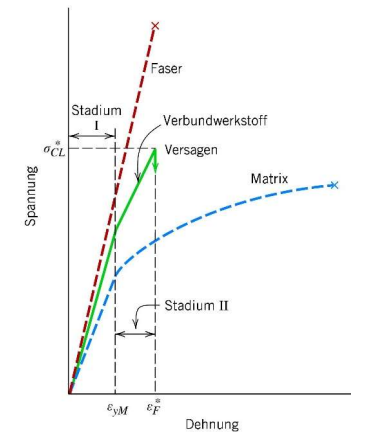
\includegraphics[width = 0.65\textwidth]{images/Materialwissenschaften/Faser_spannung-Dehnung.png}
    \caption{Spannungs-Dehnungs-Diagramm von Faser, Matrix und Verbundwerkstoff}
    \label{fig:Faser_Spannung_Dehnung}
\end{figure}
\end{addmargin}

\end{document}